%%% NOTE: I AM FIRST COMPILING MY TEX FILE IN VS Code; WILL TRANSFER CONTENT

% =====================================================================
%  Crossover disambiguation in Kuramoto-coupled dense associative
%  sequential memory.
%
%  Deck structure (as built):
%    1  Introduction   -- crossover problem; Hebbian -> Krotov DAM ->
%                         Kuramoto sequence drive; asymmetric couplings
%                         give a Lyapunov function, NOT an energy
%    2  Literature     -- foundations; the open problem
%    3  Model          -- baseline rule + algorithm; its failure at a
%                         crossover; symmetry of the Lyapunov function;
%                         heterogeneous lag-context rules
%    4  Results        -- benchmarks, catalogue, conditions, crossover
%                         resolution, superposition, robustness,
%                         findings I (rules) and II (dynamics/scaling)
%    5  Analysis       -- tensor decomposition; scalability      [Jona]
%    6  Conclusions    -- main result; applications
%    7  Open questions -- physical implementation; decaying neurons;
%                         randomly generated sequences
%
%  Remaining \TODO{} placeholders mark numbers and figures to drop in
%  from the executed notebooks.
% =====================================================================

\documentclass[aspectratio=169]{beamer}

\usetheme{Madrid}
\usecolortheme{default}

\usepackage[utf8]{inputenc}
\usepackage{amsmath, amssymb}
\usepackage{booktabs}
\usepackage{graphicx}
\graphicspath{{../}{./}}
\usepackage{algorithm}
\usepackage{algpseudocode}
\usepackage{tikz}
\usetikzlibrary{arrows.meta, positioning}

% Convenience macros used throughout (edit to taste)
\newcommand{\xxi}{\xi}
\newcommand{\thetavar}{\theta}
\newcommand{\mvar}{m}
\newcommand{\TODO}[1]{{\color{red}\textbf{[TODO: #1]}}}

\title[Kuramoto DAM: Crossover Disambiguation]{Crossover Disambiguation in Kuramoto-Coupled\\ Dense Associative Sequential Memory}
\subtitle{Learning rules for resolving branch ambiguity in phase-oscillator sequence retrieval}
\author[D. Vorobiev \and J. N\"agerl]{Daniel Vorobiev \and Jona N\"agerl}
\institute[\TODO{Institution}]{\TODO{Department / Institution}}
\date{\TODO{Date}}

\begin{document}

\begin{frame}
  \titlepage
\end{frame}

\begin{frame}{Outline}
  \tableofcontents
\end{frame}


% =====================================================================
\section[Introduction]{Introduction and Motivation}
% =====================================================================

\begin{frame}{Sequential associative memory}
  \begin{itemize}
    \item Hopfield memories store \emph{static} attractors. Motor sequences,
      speech and episodic replay require \emph{ordered} ones.
    \item Sequential retrieval $=$ a chain of transitions $\mu \to \mu+1$.
    \item \TODO{one line: hippocampal replay + phase-native hardware}
  \end{itemize}
\end{frame}

\begin{frame}{The crossover problem}
  \begin{columns}
    \begin{column}{0.55\textwidth}
      \begin{itemize}
        \item Two sequences share a contiguous run of patterns.
        \item At the shared state the network configuration is
          \emph{identical} either way: the history is not encoded in the state.
        \item Markov-1 drives both continuations equally: the branch is
          chosen by noise, not by memory.
      \end{itemize}
      \vspace{2mm}
      \centering\textbf{Can the coupling alone encode the route into $\xxi^0$?}
    \end{column}
    \begin{column}{0.45\textwidth}
      \centering
      \begin{tikzpicture}[node distance=10mm, >=Stealth]
        \node (m1) {$M_1$};
        \node (x0) [right=of m1] {$\xxi^0$};
        \node (m2) [above right=6mm and 10mm of x0] {$M_2$};
        \node (m4) [below right=6mm and 10mm of x0] {$M_4$};
        \draw[->] (m1) -- (x0);
        \draw[->, dashed, red] (x0) -- (m2) node[midway, above] {?};
        \draw[->, dashed, red] (x0) -- (m4) node[midway, below] {?};
      \end{tikzpicture}
    \end{column}
  \end{columns}
\end{frame}

\begin{frame}{Objectives}
  \begin{enumerate}
    \item A Kuramoto phase-oscillator DAM for \emph{sequences}.
    \item A learning rule that resolves crossover from the coupling alone
      --- no external gating signal.
    \item \emph{When} is disambiguation possible at all, and how robust is
      it to corruption, network size and disorder?
    \item \TODO{one line: analytical / tensor contribution}
  \end{enumerate}
\end{frame}

\begin{frame}{From Hebbian storage to dense associative memory}
  \begin{columns}[T]
    \begin{column}{0.5\textwidth}
      \textbf{Hopfield (1982)} --- pairwise Hebbian
      $J_{ij} = \frac{1}{N}\sum_\mu \xxi_i^\mu \xxi_j^\mu$:
      \[
        E = -\tfrac{N}{2}\sum_\mu \bigl(\mvar^\mu\bigr)^2 ,\quad
        \mvar^\mu = \tfrac1N \sum_j \xxi^\mu_j s_j
      \]
      Crosstalk caps capacity at $\approx 0.14N$.
    \end{column}
    \begin{column}{0.5\textwidth}
      \textbf{Krotov--Hopfield DAM (2016)} --- sharpen the nonlinearity,
      i.e.\ higher-order interactions:
      \[
        E = -\sum_\mu F\bigl(\mvar^\mu\bigr), \quad F(x) = x^{\,d+1}
      \]
      Capacity $\mathcal{O}(N^{d})$; minima sharpen with $d$.
    \end{column}
  \end{columns}
  \vspace{3mm}
  \begin{block}{Resulting drive}
    Descending $E$ gives the \emph{pure-power} drive
    $\sum_\mu \xxi_i^\mu (\mvar^\mu)^{d}$ --- one pattern index per term,
    exponent $d$ as in Krotov DAM. Every rule that follows changes only
    \emph{which} pattern each factor reads.
  \end{block}
\end{frame}

\begin{frame}{From the DAM energy to the Kuramoto sequence drive}
  \begin{enumerate}
    \item \textbf{Spins $\to$ phases:} $s_i = \cos\thetavar_i$, so
      $\dot\thetavar_i = -\partial_{\thetavar_i} E
       = \omega_i - \sin\thetavar_i \sum_\mu \xxi_i^{\mu}(\mvar^\mu)^d$.
    \item \textbf{Symmetric ($\mu \to \mu$):} true gradient flow; stored
      patterns are minima.
    \item \textbf{Asymmetric ($\mu \to \mu+1$):} drive the \emph{successor}
      (Sompolinsky--Kanter): stored patterns cease to be resting points and
      the state traverses the chain.
  \end{enumerate}
  \begin{alertblock}{Absence of an energy functional}
    Asymmetric couplings $\Rightarrow$ no potential with
    $\dot{\thetavar} = -\nabla E$. ``Minima'', ``saddles'', ``symmetry of
    the landscape'' below refer to a \textbf{Lyapunov function} of the flow.
    The absence of gradient structure is precisely what permits transitions.
  \end{alertblock}
\end{frame}


% =====================================================================
\section{Literature Review}
% =====================================================================

\begin{frame}{Foundations}
  \begin{itemize}
    \item \textbf{Hopfield (1982)} --- pairwise Hebbian attractor memory.
    \item \textbf{Krotov \& Hopfield (2016)} --- dense associative memory:
      power-$d$ interactions, super-linear capacity.
    \item \textbf{Sompolinsky \& Kanter (1986)} --- asymmetric
      $\mu \to \mu+1$ couplings turn attractors into a sequence.
    \item \textbf{Kuramoto (1975)} --- the phase-oscillator substrate.
    \item \textbf{N\"agerl \& Berloff (2025)}, arXiv:2507.21984 --- DAM in a
      higher-order Kuramoto network; the base model for this work.
    \item \TODO{oscillator / photonic hardware refs; Markov-chain sequence refs}
  \end{itemize}
\end{frame}

\begin{frame}{Open problem: crossover disambiguation}
  \begin{block}{No learning rule for crossover disambiguation}
    Existing formalisms specify \emph{how} one pattern drives the next, but
    not what happens when two sequences pass through the \emph{same} state.
  \end{block}
  \begin{itemize}
    \item A transition matrix only ever sums pure powers,
      $\sum_\beta T_{\alpha\beta}(\mvar^\beta)^d$.
    \item It cannot represent a conjunction: \emph{drive $\xxi^{\mu+1}$ only
      if $\mvar_\mu$ \textbf{and} $\mvar_{\mu-1}$ are simultaneously large.}
    \item $\Rightarrow$ gate on a \emph{product of overlaps at different
      lags}.
  \end{itemize}
\end{frame}


% =====================================================================
\section[Model]{Model and Learning Rules}
% =====================================================================

\begin{frame}{Motivation for Kuramoto dynamics}
  \begin{itemize}
    \item \textbf{Smooth retrieval.} Continuous phases resolve the traversal of a
      crossover \emph{in time}, rather than as a discrete jump.
    \item \textbf{Physical realizability.} Rules expressed purely as oscillator
      coupling are natively executable on analog and photonic hardware.
    \item \TODO{theta--gamma phase coding, if used in Applications}
  \end{itemize}
\end{frame}

\begin{frame}{Baseline rule and retrieval algorithm}
  \[
    \dot\thetavar_i = \omega_i - \sin\thetavar_i \sum_\mu
      \xxi_i^{\mu+1}\,\bigl(\mvar_i^{\mu}\bigr)^{d}, \qquad
      \mvar_i^{\mu} = \frac{1}{N-1}\sum_{j\ne i}\xxi_j^{\mu}\cos\thetavar_j
  \]
  \begin{center}
    \small Read the current overlap, drive the next pattern:
    Sompolinsky--Kanter at Krotov power $d$.
  \end{center}
  \begin{algorithm}[H]
    \small
    \begin{algorithmic}[1]
      \State cue $\thetavar(0) \gets$ (possibly corrupted) $\xxi^{0}$
      \For{each step}
        \State $\mvar^\mu_i$ for all $\mu$; \; $V_i = \sum_\mu \xxi_i^{\mu+1}(\mvar_i^\mu)^d$
        \State $\thetavar_i \mathrel{+}= dt\,(\omega_i - \sin\thetavar_i V_i)$ \; ($+$ noise)
      \EndFor
      \State decode the sequence from overlap peaks
    \end{algorithmic}
  \end{algorithm}
\end{frame}

\begin{frame}{Single-sequence retrieval, baseline rule}
  \centering
  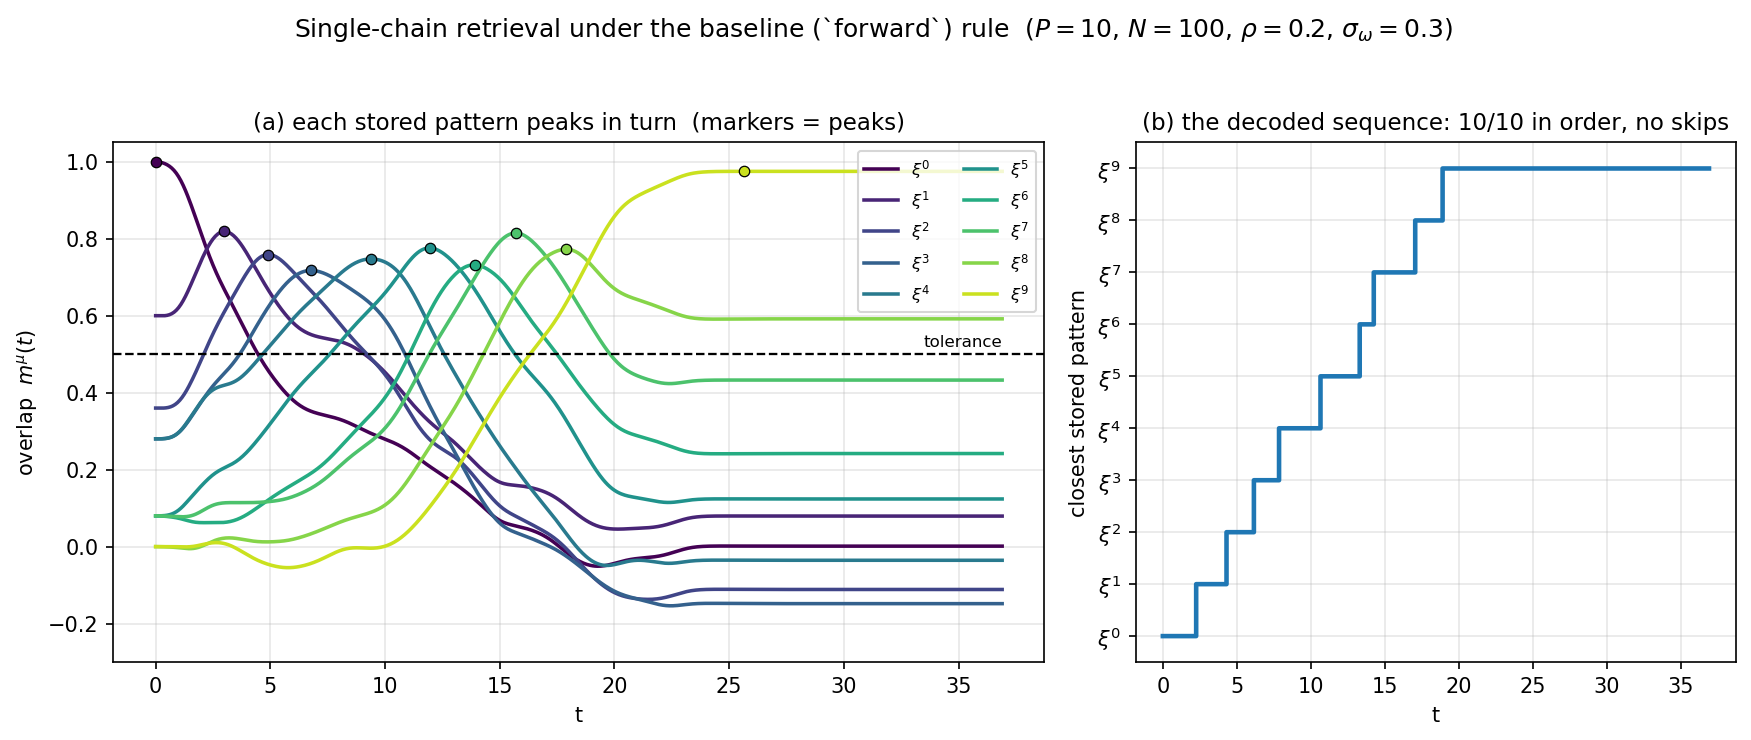
\includegraphics[height=0.68\textheight,width=\textwidth,keepaspectratio]{outputs/output.png}
  \\[1mm]
  {\small \TODO{caption: clean peak-to-peak retrieval through $P$ patterns}}
\end{frame}

\begin{frame}{Baseline rule at a crossover}
  \centering
  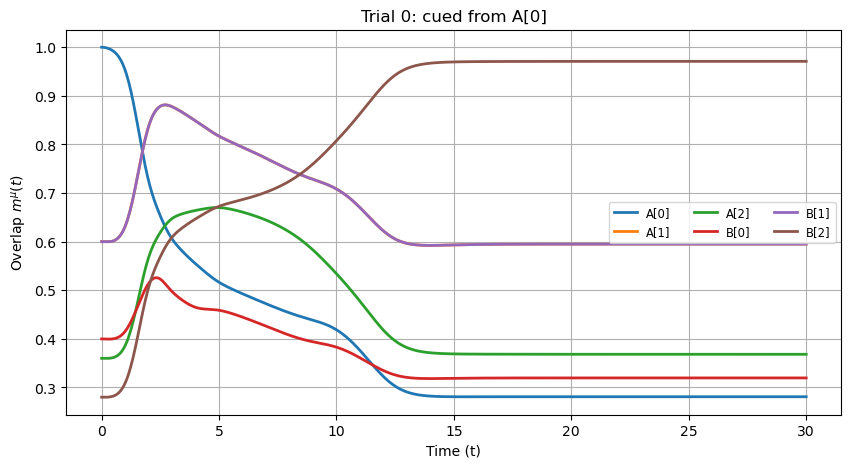
\includegraphics[height=0.62\textheight,width=0.8\textwidth,keepaspectratio]{outputs/crossover_vanilla.png}
  \\[1mm]
  {\small Both continuations rise together out of the shared state.
  Branch choice at chance: \TODO{XX\%} vs.\ $50\%$.}
\end{frame}

\begin{frame}{Innate symmetry of the Lyapunov function}
  \begin{itemize}
    \item Couplings are asymmetric $\Rightarrow$ no energy; the flow is
      organized by a Lyapunov function $V$ built from the same pure powers.
    \item Every term of $V$ reads \emph{one} pattern index --- nothing in it
      records \emph{how} the state reached the shared pattern.
    \item At $\xxi^\star$ the gate depends only on $\mvar(\xxi^\star)$, identical
      for both branches: the two exits are related by an exact symmetry of
      $V$ (a degenerate saddle).
    \item[$\Rightarrow$] The symmetry must be broken by information the
      current state cannot carry: overlaps at \emph{several lags},
      multiplied rather than summed within a single term.
  \end{itemize}
\end{frame}

\begin{frame}{Heterogeneous lag-context rules}
  \[
    \dot\thetavar_i = \omega_i - \sin\thetavar_i \sum_{\mu}\sum_{\text{terms}}
      w \;\xxi_i^{\mu+s} \prod_{l \in \text{lags}} \mvar_i^{\mu - l}
  \]
  \begin{itemize}
    \item A rule is a \emph{table of terms}: target offset $s$, $d$ source
      lags, weight $w$. Lags $(0,0,0)$ recovers the forward rule.
    \item Different lags in one term $\Rightarrow$ the gate encodes
      \emph{which branch} produced the current state.
  \end{itemize}
\end{frame}


% =====================================================================
\section[Results]{Numerical Experiments and Results}
% =====================================================================

\begin{frame}{Benchmarks}
  \centering
  \small
  \begin{tabular}{llccl}
    \toprule
    Tag & Geometry & $P$ & Shared run $L$ & Reach needed \\
    \midrule
    \texttt{2-1-2} & one shared pattern   & 5 & 1 & 1 \\
    \texttt{2-2-2} & shared segment       & 6 & 2 & 2 \\
    \texttt{2-3-2} & failure case         & 7 & 3 & 3 (beyond catalogue) \\
    \bottomrule
  \end{tabular}
  \\[3mm]
  \begin{itemize}
    \item \textbf{Scoring:} every \emph{unshared} pattern of the cued branch
      decoded, in order. Shared positions carry no rule information and are
      excluded.
    \item \textbf{Branch diagnostic:} correct vs.\ incorrect drive at the
      exit; separates incorrect selection from correct selection without
      lock-on.
  \end{itemize}
\end{frame}

\begin{frame}{Catalogue of learning rules}
  \centering
  \small
  \begin{tabular}{lll}
    \toprule
    Rule & Gate at pattern $\mu$ & Reach \\
    \midrule
    \texttt{self} & $\xxi^\mu \mvar_\mu^3$ & 0 (control) \\
    \texttt{forward} (baseline) & $\xxi^{\mu+1} \mvar_\mu^3$ & 0 \\
    \texttt{skip-two} & $\xxi^{\mu+2} \mvar_\mu^3$ & 0 \\
    \texttt{bigram} & $\xxi^{\mu+1} \mvar_\mu |\mvar_{\mu-1}|^2$ & 1 \\
    \texttt{multilag} & $\xxi^{\mu+1} \mvar_\mu \sum_k w_k |\mvar_{\mu-k}|^2$ & $\le K$ \\
    \texttt{coh bigram} & $\xxi^{\mu+1} \mvar_\mu^2 \mvar_{\mu-1}$ & 1 \\
    \texttt{coh trigram} & $\xxi^{\mu+1} \mvar_\mu \mvar_{\mu-1} \mvar_{\mu-2}$ & 2 \\
    \bottomrule
  \end{tabular}
  \\[3mm]
  {\small Reach $\ge L$ is required to access \emph{any} unshared
  information: necessary, not sufficient.}
\end{frame}

\begin{frame}{Experimental conditions}
  \begin{itemize}
    \item $d = 3$; corruption ratio $\rho$ sets consecutive-pattern overlap
      to exactly $1-2\rho$.
    \item $\omega_i \sim \mathcal{N}(\mu_\omega, \sigma_\omega^2)$ ---
      required to break the exact-cue degeneracy.
    \item Euler / Euler--Maruyama, step $dt$, stationary early-stop.
    \item \textbf{Proportional gain:} rescale each term by
      $(1-2\rho)^{-\sum \text{lags}}$ to undo the geometric decay of lagged
      overlaps. Both raw and gain-corrected catalogues are evaluated.
    \item \TODO{values: $N$, $P$, $\rho$, $dt$, $T$, trials, tolerance}
  \end{itemize}
\end{frame}

\begin{frame}{Crossover resolution}
  \begin{itemize}
    \item \texttt{forward}: at chance on branch choice; it commits rapidly,
      to the incorrect branch in half of trials.
    \item Context rules: well above chance, but frequently trade
      completeness for it --- lagged factors leave fewer for
      self-amplification.
    \item \texttt{coh bigram} keeps two factors on the current overlap
      ($\mvar_\mu^2 \mvar_{\mu-1}$): it both selects the correct branch and commits
      to it.
    \item \TODO{outcome + branch-choice bar charts, per geometry}
  \end{itemize}
\end{frame}

\begin{frame}{Superposition of rules}
  \begin{itemize}
    \item Mixing two context rules at weight $w$ trades commitment against
      branch information continuously.
    \item \texttt{multilag} $(w_0,w_1,w_2)$: $w_0$ controls commitment,
      $w_1,w_2$ supply branch information.
    \item \TODO{mixture sweep grid}
  \end{itemize}
\end{frame}

\begin{frame}{Robustness: corruption ratio and network size}
  \centering
  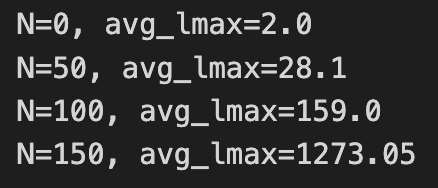
\includegraphics[height=0.58\textheight,width=0.62\textwidth,keepaspectratio]{outputs/large_N.png}
  \\[1mm]
  {\small \TODO{caption: retrieval rate vs.\ $\rho$ and vs.\ $N$, per rule;
  breakdown point $=$ largest $\rho N$ with rate $\ge 50\%$}}
\end{frame}

\begin{frame}{Findings I: learning rules}
  \begin{itemize}
    \item \textbf{Reach $\ge L$ is necessary, not sufficient.} The
      discriminating signal is a \emph{dynamic residual} between traversed
      and untraversed predecessor; it decays within $\sim 2$ steps.
    \item \textbf{Commitment against branch information} is the governing
      trade-off; \TODO{best rule} achieves the best balance.
    \item \textbf{Gain correction is not uniformly beneficial:} it recovers
      the hardest geometry while destabilizing rules that already succeeded.
    \item \textbf{No rule resolves $L \gtrsim 3$}, and uncorrelated random
      patterns give $0\%$ for \emph{every} rule: sequential similarity
      structure is a prerequisite for all rules tested.
  \end{itemize}
\end{frame}

\begin{frame}{Findings II: dynamics and scaling}
  \begin{itemize}
    \item \textbf{U-shaped dependence on the corruption ratio.} Retrieval
      peaks at intermediate $\rho$ and degrades in \emph{both} directions.
      \begin{itemize}
        \item[--] \emph{Small} Hamming distance: patterns are near-duplicates
          and their overlaps differ by thousandths. In such a tightly packed
          Lyapunov landscape the rules cannot separate them.
        \item[--] \emph{Large} $\rho$: consecutive overlaps are too small to
          sustain the cascade.
      \end{itemize}
    \item \textbf{Frequency disorder and noise are necessary.} At
      $\omega \equiv 0$ an exact cue satisfies $\sin\thetavar_i = 0$ for all
      $i$: the drive vanishes identically and the system stalls at the cue.
    \item \textbf{Network size and frequency disorder must be scaled
      jointly.} Larger $N$ stores more patterns with less crosstalk, but as
      the overlaps concentrate a fixed $\sigma_\omega$ crosses the rules'
      disorder tolerance and retrieval collapses. Two equivalent remedies:
      reduce $\sigma_\omega$ as $N$ grows, or hold it and raise the drive
      with the proportional-gain filter.
  \end{itemize}
\end{frame}


% =====================================================================
\section[Analysis]{Theoretical Analysis}
% =====================================================================

\begin{frame}{Tensor structure: symmetric vs.\ asymmetric}
  \begin{itemize}
    \item \TODO{write the coupling as $J_i^{\mu_1\dots\mu_d,\nu}$ and split
      it under permutation of the read indices}
    \item \TODO{forward rule $=$ fully symmetric (pure-power) part;
      lag-context rules $=$ mixed-symmetry part}
    \item \TODO{what the decomposition yields: stability conditions, or a
      clean statement of the reach requirement}
  \end{itemize}
\end{frame}

\begin{frame}{Scalability}
  \begin{itemize}
    \item \TODO{cost per step: $\mathcal{O}(KPN)$ buffer $+$
      $\mathcal{O}(\text{terms}\times N)$ drive}
    \item \TODO{capacity in $N$, $d$ --- do context terms cost capacity?}
    \item \TODO{Jona: scaling law / bound}
  \end{itemize}
\end{frame}


% =====================================================================
\section[Conclusions]{Conclusions and Outlook}
% =====================================================================

\begin{frame}{Conclusions}
  \begin{block}{Main result}
    To resolve branching after a shared segment, the learning rule needs a
    \textbf{lag reference exceeding the length of the shared segment.} Only a
    factor reading back past the last shared pattern breaks the innate
    symmetry of the Lyapunov function; rules whose lags all sit inside the
    shared run are symmetric in the branches by construction.
  \end{block}
  \begin{itemize}
    \item Markov-1 Kuramoto DAM retrieves single sequences reliably, but its
      Lyapunov function is symmetric at every shared state, leaving the
      branch choice to noise.
    \item Sufficient reach is necessary, not sufficient: commitment and
      branch information trade off.
    \item The operating point is set by $\rho$, $N$ and $\sigma_\omega$
      \emph{together}, not by the rule alone.
  \end{itemize}
\end{frame}

\begin{frame}{Applications}
  \begin{itemize}
    \item \textbf{Physical simulators.} Every rule is pure oscillator
      coupling, and therefore maps onto analog and photonic Kuramoto
      hardware: crossover-resolving memory as a physical primitive.
    \item \textbf{Neurobiology.} \TODO{phase-coded replay, theta--gamma;
      lag-context gating as a disambiguation mechanism}
    \item \TODO{motor-sequence chaining, time-series disambiguation}
  \end{itemize}
\end{frame}


% =====================================================================
\section[Open Questions]{Active Questions for Further Investigation}
% =====================================================================

\begin{frame}{Active questions}
  \begin{enumerate}
    \item How are these learning rules implemented in \textbf{physical
      (oscillator-based) simulators}?
    \item What is the role of \textbf{decaying neurons}, and can they
      replace the explicit lag buffer?
    \item How does one generate \textbf{robust rules for randomly generated
      pattern sequences}?
  \end{enumerate}
  \vspace{3mm}
  {\small Further open questions: whether the resolvable shared-run length
  $L$ admits a fundamental ceiling, and whether rule weights can be
  \emph{learned} rather than constructed by hand.}
\end{frame}

\begin{frame}{Question 1: physical implementation}
  \begin{itemize}
    \item Rules are rank-$(d{+}1)$ couplings; hardware (Ising machines, OPO
      and polariton networks, CMOS oscillatory NNs) gives \emph{pairwise}.
      Which mechanism synthesizes the product: ancilla modes, parametric
      mixing, or measurement feedback?
    \item Can the lagged factor $\mvar_{\mu-\ell}$ be a physical \emph{delay
      line} rather than a stored buffer? This would render the rule local
      in time as well as in space.
    \item \TODO{required coupling precision and noise floor before branch
      choice falls to chance}
  \end{itemize}
\end{frame}

\begin{frame}{Question 2: decaying neurons}
  \begin{itemize}
    \item Replace the discrete lag by a decaying trace
      $\tau \dot h_\mu = -h_\mu + |\mvar_\mu|^2$. Adaptation achieves the same
      from the opposite direction: the active pattern suppresses itself and
      releases the flow to its successor.
    \item Open: whether a single time constant $\tau$ provides reach beyond
      the shared segment, and whether it is simpler to realize physically
      than a multi-lag product.
  \end{itemize}
  \begin{block}{Selected references}
    \footnotesize
    \textbf{Delayed / slow synapses:} Sompolinsky \& Kanter (PRL 57, 2861,
    1986); Kleinfeld (PNAS 83, 9469, 1986); Tank \& Hopfield (PNAS 84, 1896,
    1987).
    \textbf{Adaptation-driven transitions:} Horn \& Usher (Phys.\ Rev.\ A 40,
    1036, 1989); Herrmann, Ruppin \& Usher (Biol.\ Cybern.\ 68, 455, 1993);
    Treves (Cogn.\ Neuropsych.\ 22, 276, 2005) --- latching; Recanatesi et
    al.\ (Front.\ Comput.\ Neurosci.\ 9:149, 2015); Gillett, Pereira \&
    Brunel (PNAS 117, 29948, 2020).
    \textbf{Closest precedent:} Martinez Mayorquin et al.\ (ICANN 2019,
    pp.\ 793--805) --- filtered synaptic traces for \emph{sequence
    disambiguation}.
  \end{block}
\end{frame}

\begin{frame}{Question 3: randomly generated sequences}
  \begin{itemize}
    \item Uncorrelated patterns: $0\%$ retrieval for every rule, raw and
      gain-corrected --- peak overlaps $0.16$--$0.19$ against a $0.5$
      tolerance.
    \item Gating failure, not drive failure: for independent patterns
      $\mvar_{\mu-\ell} = \mathcal{O}(N^{-1/2})$; rescaling a gate that reads
      $\mvar \approx 0$ has no effect.
    \item To test: whitened / pseudo-inverse storage (Chaudhry et al.,
      \emph{Long Sequence Hopfield Memory}); larger $d$; ridge-fitted
      weights as an upper-bound control.
    \item \TODO{retrieval rate vs.\ pattern correlation, mutation chain
      $\to$ fully random: locate the collapse threshold per rule}
  \end{itemize}
\end{frame}

\begin{frame}
  \centering
  \Large Thank you \\[2mm]
  \normalsize \TODO{contact / repo QR}
\end{frame}

\end{document}
